\section*{Problem No.4} \label{sec:prob4}
Figure \ref{fig:fig4_ab} shows the image along with the distribution of its singular value. The distribution shows a single spike which rapidly smooth out. We think this is due to the greater intensity along the nose of the \emph{mandrill}. 

\begin{figure}[tbh]
\centering        
   \subfloat [\emph{mandrill} image] {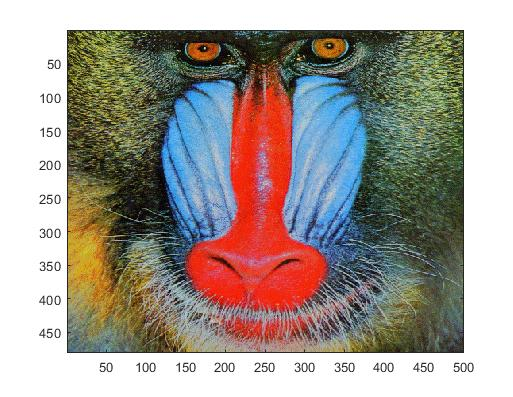
\includegraphics[width=0.5\textwidth]{p4/p4_a.jpg}}
   \subfloat [distribution of singular values]{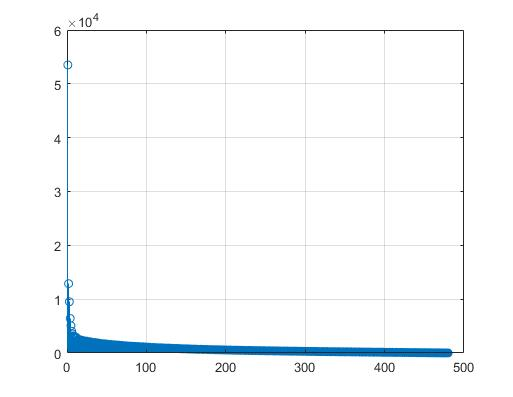
\includegraphics[width=0.5\textwidth]{p4/p4_b.jpg}}
   \caption{ The image (left) along with the distribution of its singular values (right).}
   \label{fig:fig4_ab}
\end{figure}


Figure \ref{fig:fig4_c} shows approximation of the image using rank \emph{k} approximation based on SVD. As the rank increases, more details appears as we are extracting more details using the largest singular value then the second largest and so on. 

Figure \ref{tab:error} shows the relative and absolute error of the rank \emph{k} approximation. As it was suggest from Figure \ref{fig:fig4_c}, increasing the rank reduces the error. While increasing the rank from 1 to 6 decreased the error by third, moving to higher ranks does not scale the same which suggests (at least for this example) that using fewer columns of SVD can approximate the image well. 
 
\begin{figure}[tbh]
\centering        
   \subfloat {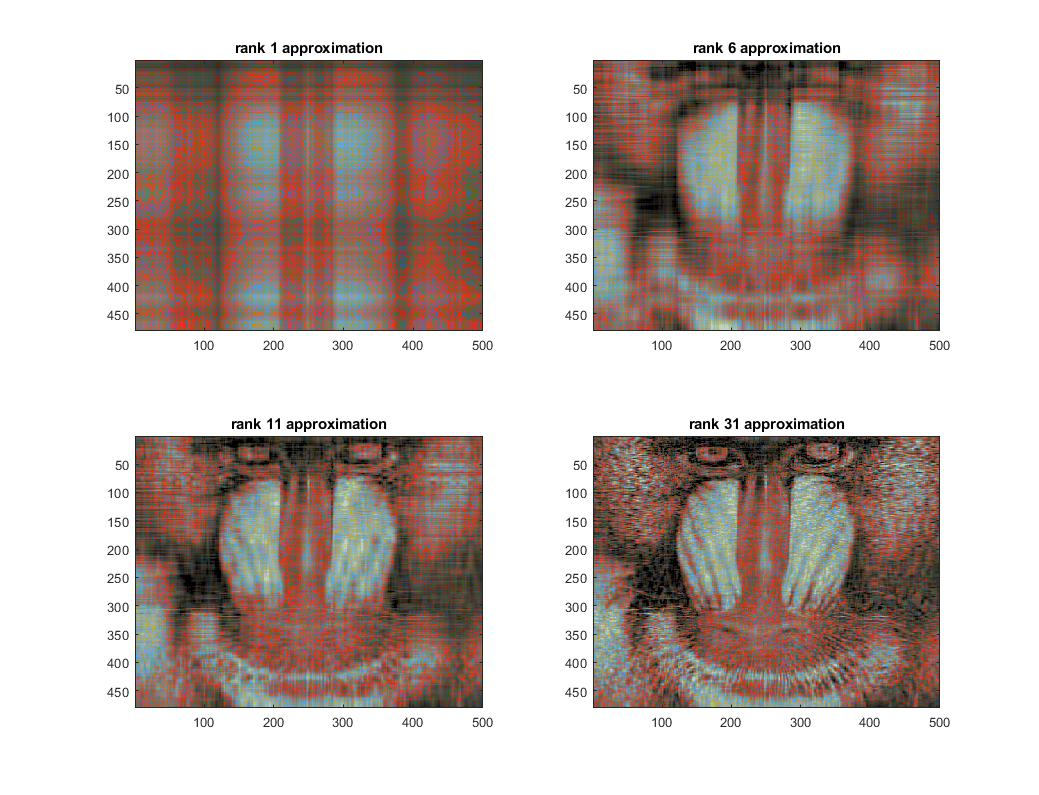
\includegraphics[width=0.95\textwidth]{p4/p4_c.jpg}}
   \caption{Four different approximation for the image based on the rank. }
   \label{fig:fig4_c}
\end{figure}

\begin{figure}[tbh]
 \centering    
\begin{tabular}{ |p{5cm}|| p{3cm}|p{3cm}|}
 \hline
 & Absolute Error &  Relative Error \\ \hhline{|=|=|=|}
 \hline
 Rank 1 approximation  & $12891.1649$ & $1.2699e^{-15}$    \\
 Rank 6 approximation  & $3537.8836$  & $6.4268e^{-16}$   \\
 Rank 11 approximation & $2820.0648$  & $6.4502e^{-16}$   \\
 Rank 31 approximation & $1985.461 $  & $4.5808e^{-16}$   \\
 \hline
\end{tabular} 
\caption{The absolute error (norm) along with relative error of the approximation of  image based of the rank.}
   \label{tab:error}
\end{figure} 